%%%%%%%%%%%%%%%%%%%%%%%%%%%%%%%%%%%%%%%%%%%%%%%%%%%%%%%%%%%%%%%%%%%%%%%%%%%%%%%%%%
\begin{frame}[fragile]\frametitle{}
\begin{center}
{\Large ChatGPT (Open AI)}
\end{center}
\end{frame}



%%%%%%%%%%%%%%%%%%%%%%%%%%%%%%%%%%%%%%%%%%%%%%%%%%%%%%%%%%%
\begin{frame}[fragile]\frametitle{Open AI}


\begin{itemize}
\item San Francisco-based artificial intelligence company
\item Famous for its well-known DALL·E, a deep-learning model that generates images from text instructions called prompts.
\item OpenAI Inc. is the non-profit parent company of the for-profit OpenAI LP.
\item Initially supported by Elon Musk
\item The CEO is Sam Altman, who previously was president of Y Combinator.
\item Microsoft is a partner and investor in the amount of \$1 billion dollars. They jointly developed the Azure AI Platform.
\item Mission: To ensure that artificial general intelligence benefits all of humanity
\item Prevent misuse of AI
\end{itemize}	 

\end{frame}

%%%%%%%%%%%%%%%%%%%%%%%%%%%%%%%%%%%%%%%%%%%%%%%%%%%%%%%%%%%
\begin{frame}[fragile]\frametitle{What is ChatGPT?}


\begin{itemize}
\item A Chatbot
\item A language model, that takes 'prompt' from user and generates a response.
\item Built by OpenAI
\item Released in Nov 2022
\item Got 1m users in 5 days  (Insta 2.5 months, Spotify 5m, Facebook 10m, Netflix 3.5yrs)
\end{itemize}	 

			\begin{center}
			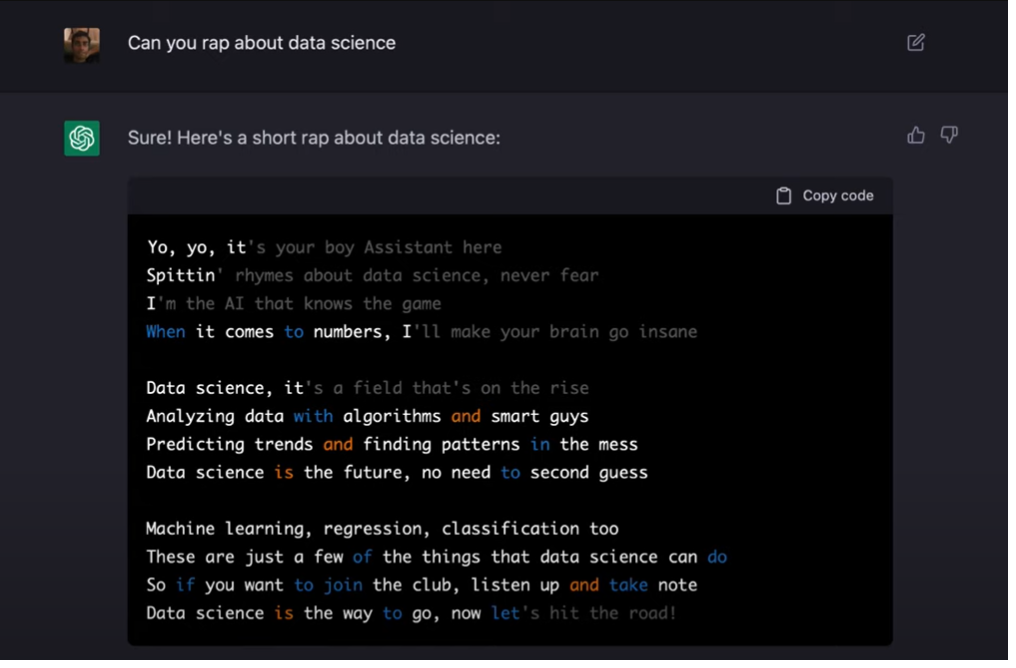
\includegraphics[width=0.6\linewidth,keepaspectratio]{chatgpt8}
			\end{center}		
			
			
			{\tiny (Ref: ChatGPT - Explained! - CodeEmporium)}
			
			
\end{frame}

%%%%%%%%%%%%%%%%%%%%%%%%%%%%%%%%%%%%%%%%%%%%%%%%%%%%%%%%%%%
\begin{frame}[fragile]\frametitle{What is ChatGPT?}


\begin{itemize}
\item GPT based
\item Trained on large amount of data
\item Uses Supervised Learning and Reinforcement Learning.
\item Gives answers like a human
\item Can ask Follow-up questions and even admit mistakes.
\end{itemize}	 

\end{frame}

%%%%%%%%%%%%%%%%%%%%%%%%%%%%%%%%%%%%%%%%%%%%%%%%%%%%%%%%%%%
\begin{frame}[fragile]\frametitle{Prerequisites: What is Reinforcement Learning (RL)?}


\begin{itemize}
\item RL is a method of achieving a goal via rewards. Find best path to get maximum points (game below)
\item Agent: Makes the moves
\item Reward: Positive or Negative (as shown)
\item State: Current position, location.
\item Action: Move done by the Agent
\item Policy: Sequence of Actions that Agent takes to achieve the goal, say, Down-Down-Right-Right-Right (reward 6)..there could be other paths and one(or more) of then can be the best.
\end{itemize}	 


			\begin{center}
			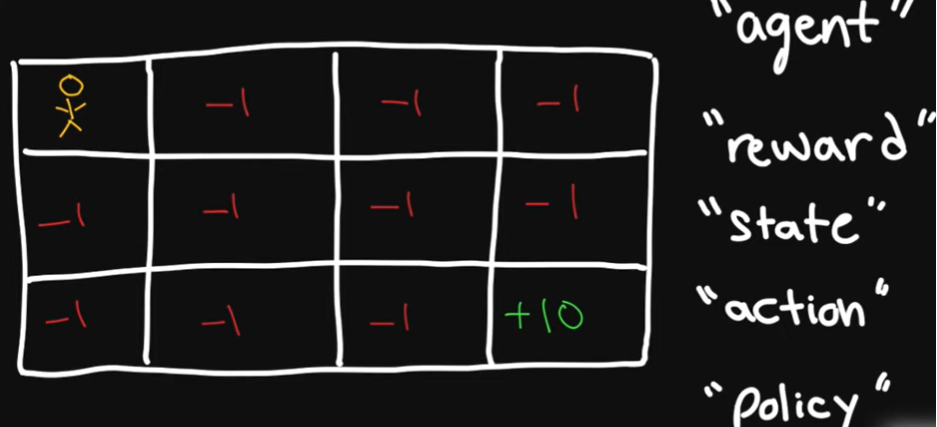
\includegraphics[width=0.6\linewidth,keepaspectratio]{chatgpt9}
			\end{center}		
			
			
			{\tiny (Ref: ChatGPT - Explained! - CodeEmporium)}
\end{frame}

%%%%%%%%%%%%%%%%%%%%%%%%%%%%%%%%%%%%%%%%%%%%%%%%%%%%%%%%%%%
\begin{frame}[fragile]\frametitle{RL in context of ChatGPT}


\begin{itemize}
\item Agent: the model, it spits out words
\item Reward: score at predicting each next word
\item State: prompt + sentence generated so far
\item Action: Predicting the next word
\item Policy: Sequence of words and then total rewards for them.
\item Manual person can chose between such sequences (or polices) and label which is best. Then PPO can happen to adjust backwardly the reward function.
\item So, the Reinforcement Learning is used to capture human preferences and reduce misalignment.
\end{itemize}	 
\end{frame}



%%%%%%%%%%%%%%%%%%%%%%%%%%%%%%%%%%%%%%%%%%%%%%%%%%%%%%%%%%%
\begin{frame}[fragile]\frametitle{GPTs Series}


\begin{itemize}
\item GPT + Generative Pre-trained Transformers
\item GPT-1, GPT-2 and GPT-3 are similar in terms of architecture 
\item Differ on the data and the number of transformer blocks with the number of incoming tokens.   
\item GPT-1 : 12 blocks, encoded using a Byte pair encoding, 512 tokens: 117 million parameters 
\item GPT-2 : 48 blocks, 1024 tokens: 1.5 billion parameters 
\item GPT-3 : 96 blocks, 2048 tokens: 175 billion parameters 
\end{itemize}	 

\end{frame}

%%%%%%%%%%%%%%%%%%%%%%%%%%%%%%%%%%%%%%%%%%%%%%%%%%%%%%%%%%%
\begin{frame}[fragile]\frametitle{GPTs Trainings}


\begin{itemize}
\item GPT-1 is trained in a self-supervised manner (learn to predict the next word in text data) and fine-tuned in a supervised learning manner. 
\item GPT-2 is trained in a fully self supervised way, focusing on zero-shot transfer
\item  GPT-3 is pre-trained in a self supervised manner exploring a bit more the few-shots fine-tuning.
\item GPT-1 is pre-trained on the BooksCorpus dataset, containing ~7000 books amounting to ~5GB of data
\item GPT-2 is pre-trained using the WebText dataset which is a more diverse set of internet data containing ~8M documents for about ~40 GB of data
\item GPT-3 uses an expanded version of the WebText dataset, two internet-based books corpora that are not disclosed and the English-language Wikipedia which constituted ~600 GB (45TB?) of data
\end{itemize}	 

\end{frame}



%%%%%%%%%%%%%%%%%%%%%%%%%%%%%%%%%%%%%%%%%%%%%%%%%%%%%%%%%%%
\begin{frame}[fragile]\frametitle{Misalignment Issue}


\begin{itemize}
\item GPT-3 was trained to predict the next word. Not much of context there.
\item Introducing prompting : provide with certain samples and context

\end{itemize}	 

			\begin{center}
			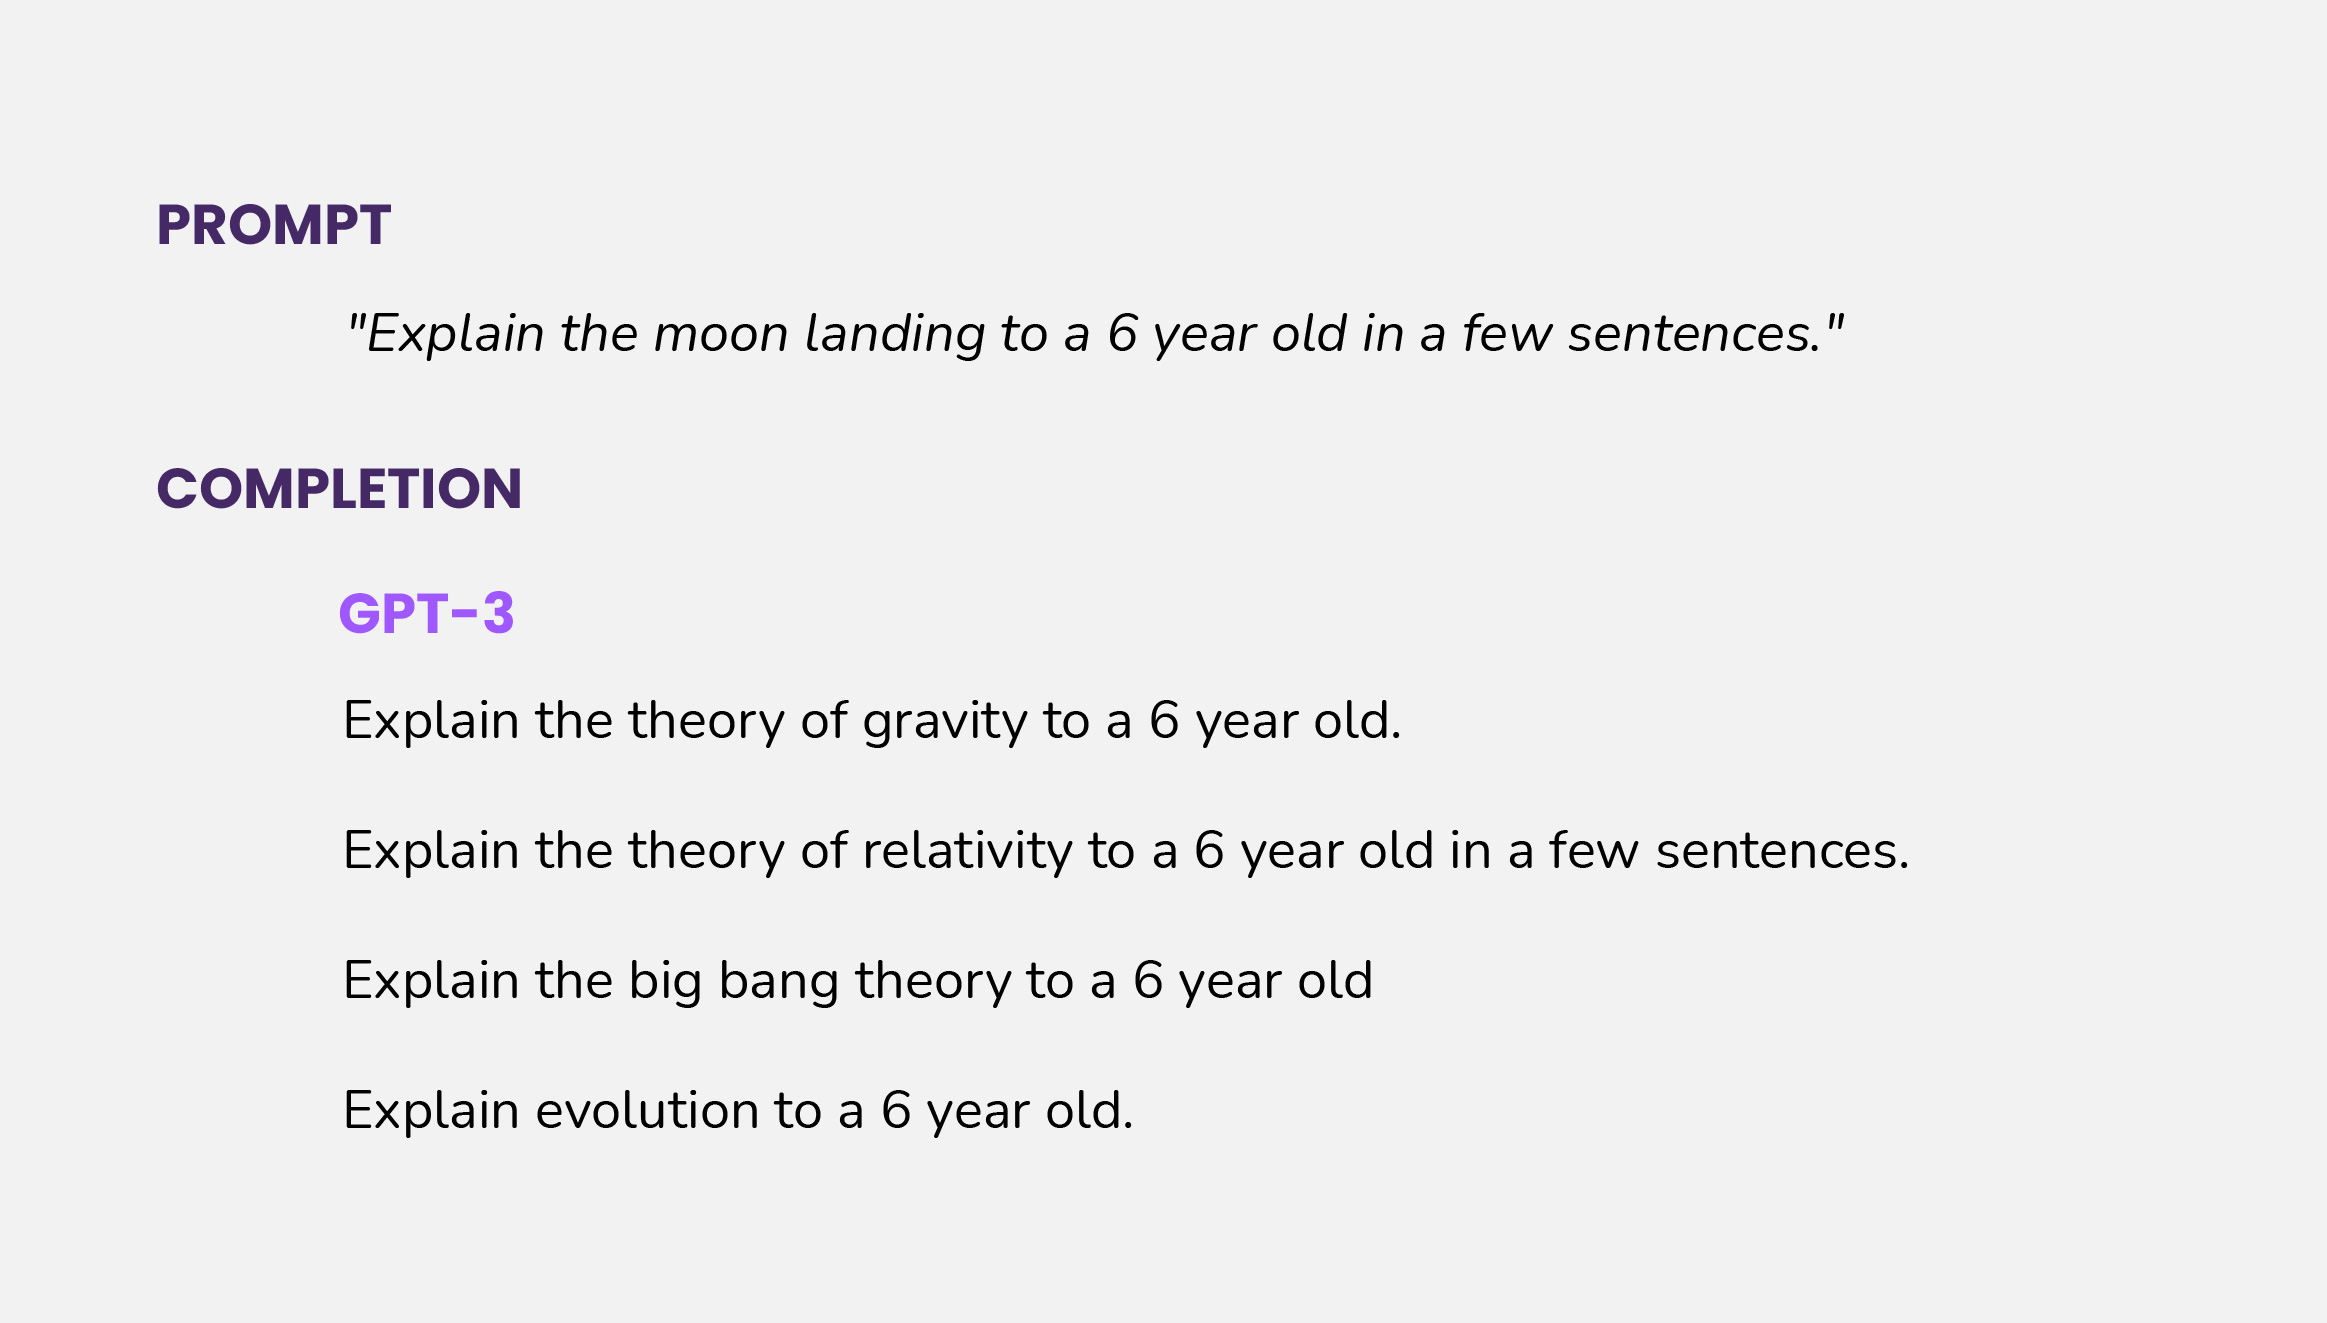
\includegraphics[width=0.6\linewidth,keepaspectratio]{chatgpt2}
			
			{\tiny "Example of misalignment between text to be predicted and final use"}
			\end{center}		
			
			
			{\tiny (Ref: ChatGPT: training process, advantages, and limitations - By Sergio Soage, Machine Learning Engineer at Aivo)}
			
\end{frame}

%%%%%%%%%%%%%%%%%%%%%%%%%%%%%%%%%%%%%%%%%%%%%%%%%%%%%%%%%%%
\begin{frame}[fragile]\frametitle{Curated Training Data}


\begin{itemize}
\item To fix this misalignment, humans must be involved in teaching GPT, and in this way, GPT will be able to generate better questions as it evolves.
\end{itemize}	 

			\begin{center}
			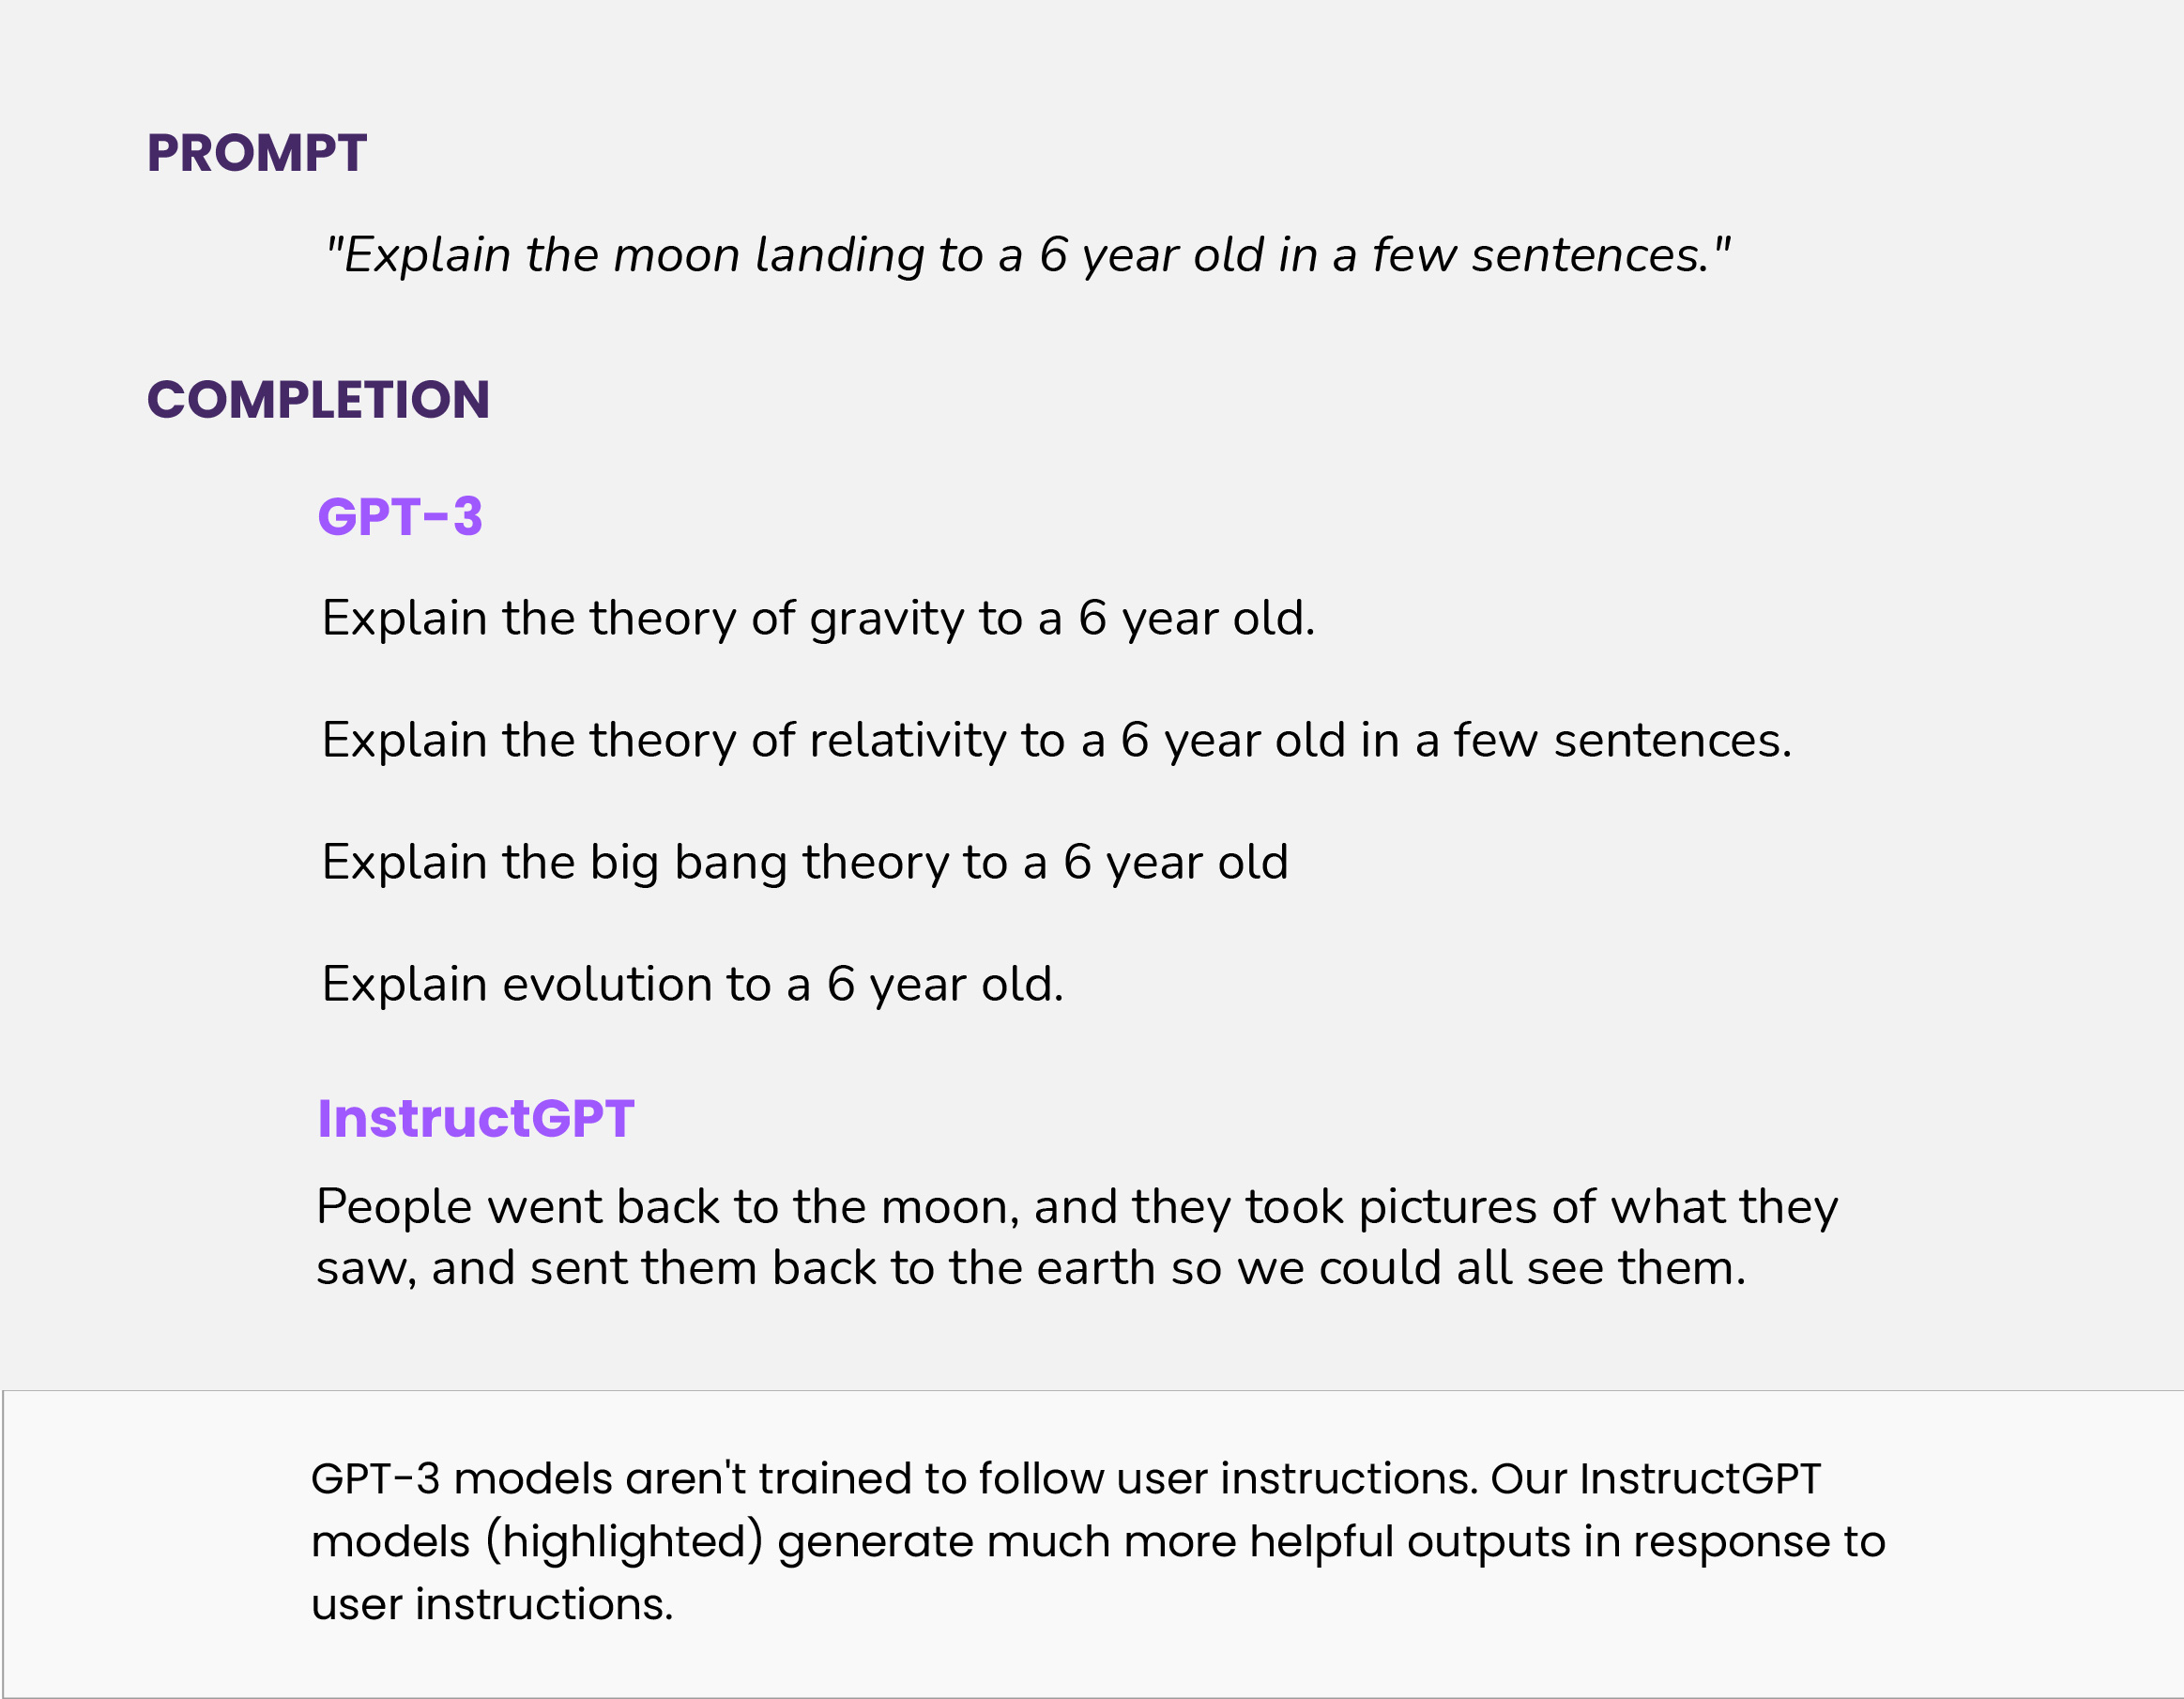
\includegraphics[width=0.6\linewidth,keepaspectratio]{chatgpt3}
			
			\end{center}		
			
			{\tiny (Ref: ChatGPT: training process, advantages, and limitations - By Sergio Soage, Machine Learning Engineer at Aivo)}
			
\end{frame}


%%%%%%%%%%%%%%%%%%%%%%%%%%%%%%%%%%%%%%%%%%%%%%%%%%%%%%%%%%%
\begin{frame}[fragile]\frametitle{Better GPT 3.5}

\begin{itemize}
\item GPT-3.5 = Better of GPT-3 and sibling model InstructGPT + training(manually labeled data + reinforcement learning)
\item GPT-3.0’s answer is short and common but InstructGPT gives answers that the users prefer.
\end{itemize}	 
			\begin{center}
			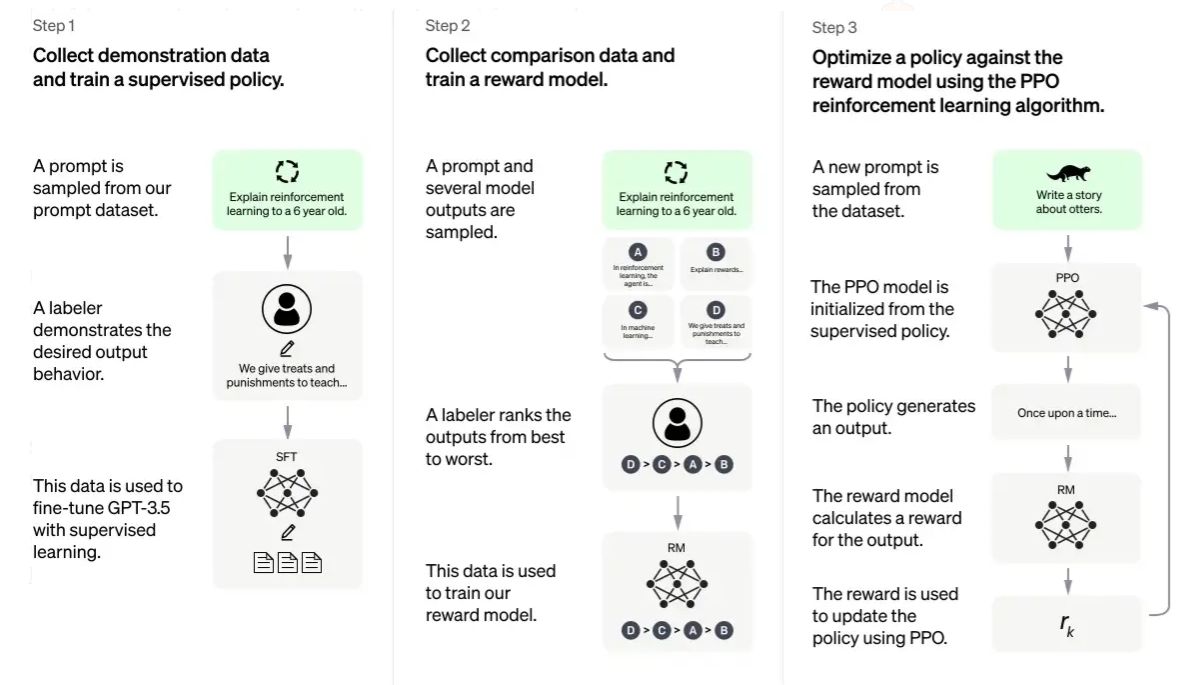
\includegraphics[width=0.8\linewidth,keepaspectratio]{chatgpt1}
			\end{center}		
			
			\tiny{(Ref: https://openai.com/blog/chatgpt/)}
\end{frame}

%%%%%%%%%%%%%%%%%%%%%%%%%%%%%%%%%%%%%%%%%%%%%%%%%%%%%%%%%%%
\begin{frame}[fragile]\frametitle{Step 1}

\begin{itemize}
\item Have a prompts dataset 
\item Let human laborer get the correct response for them
\item Do fine-tuning of GPT 3.5 using this data via supervised learning (SFT). 
\item Simple but very expensive.
\end{itemize}	 

			\begin{center}
			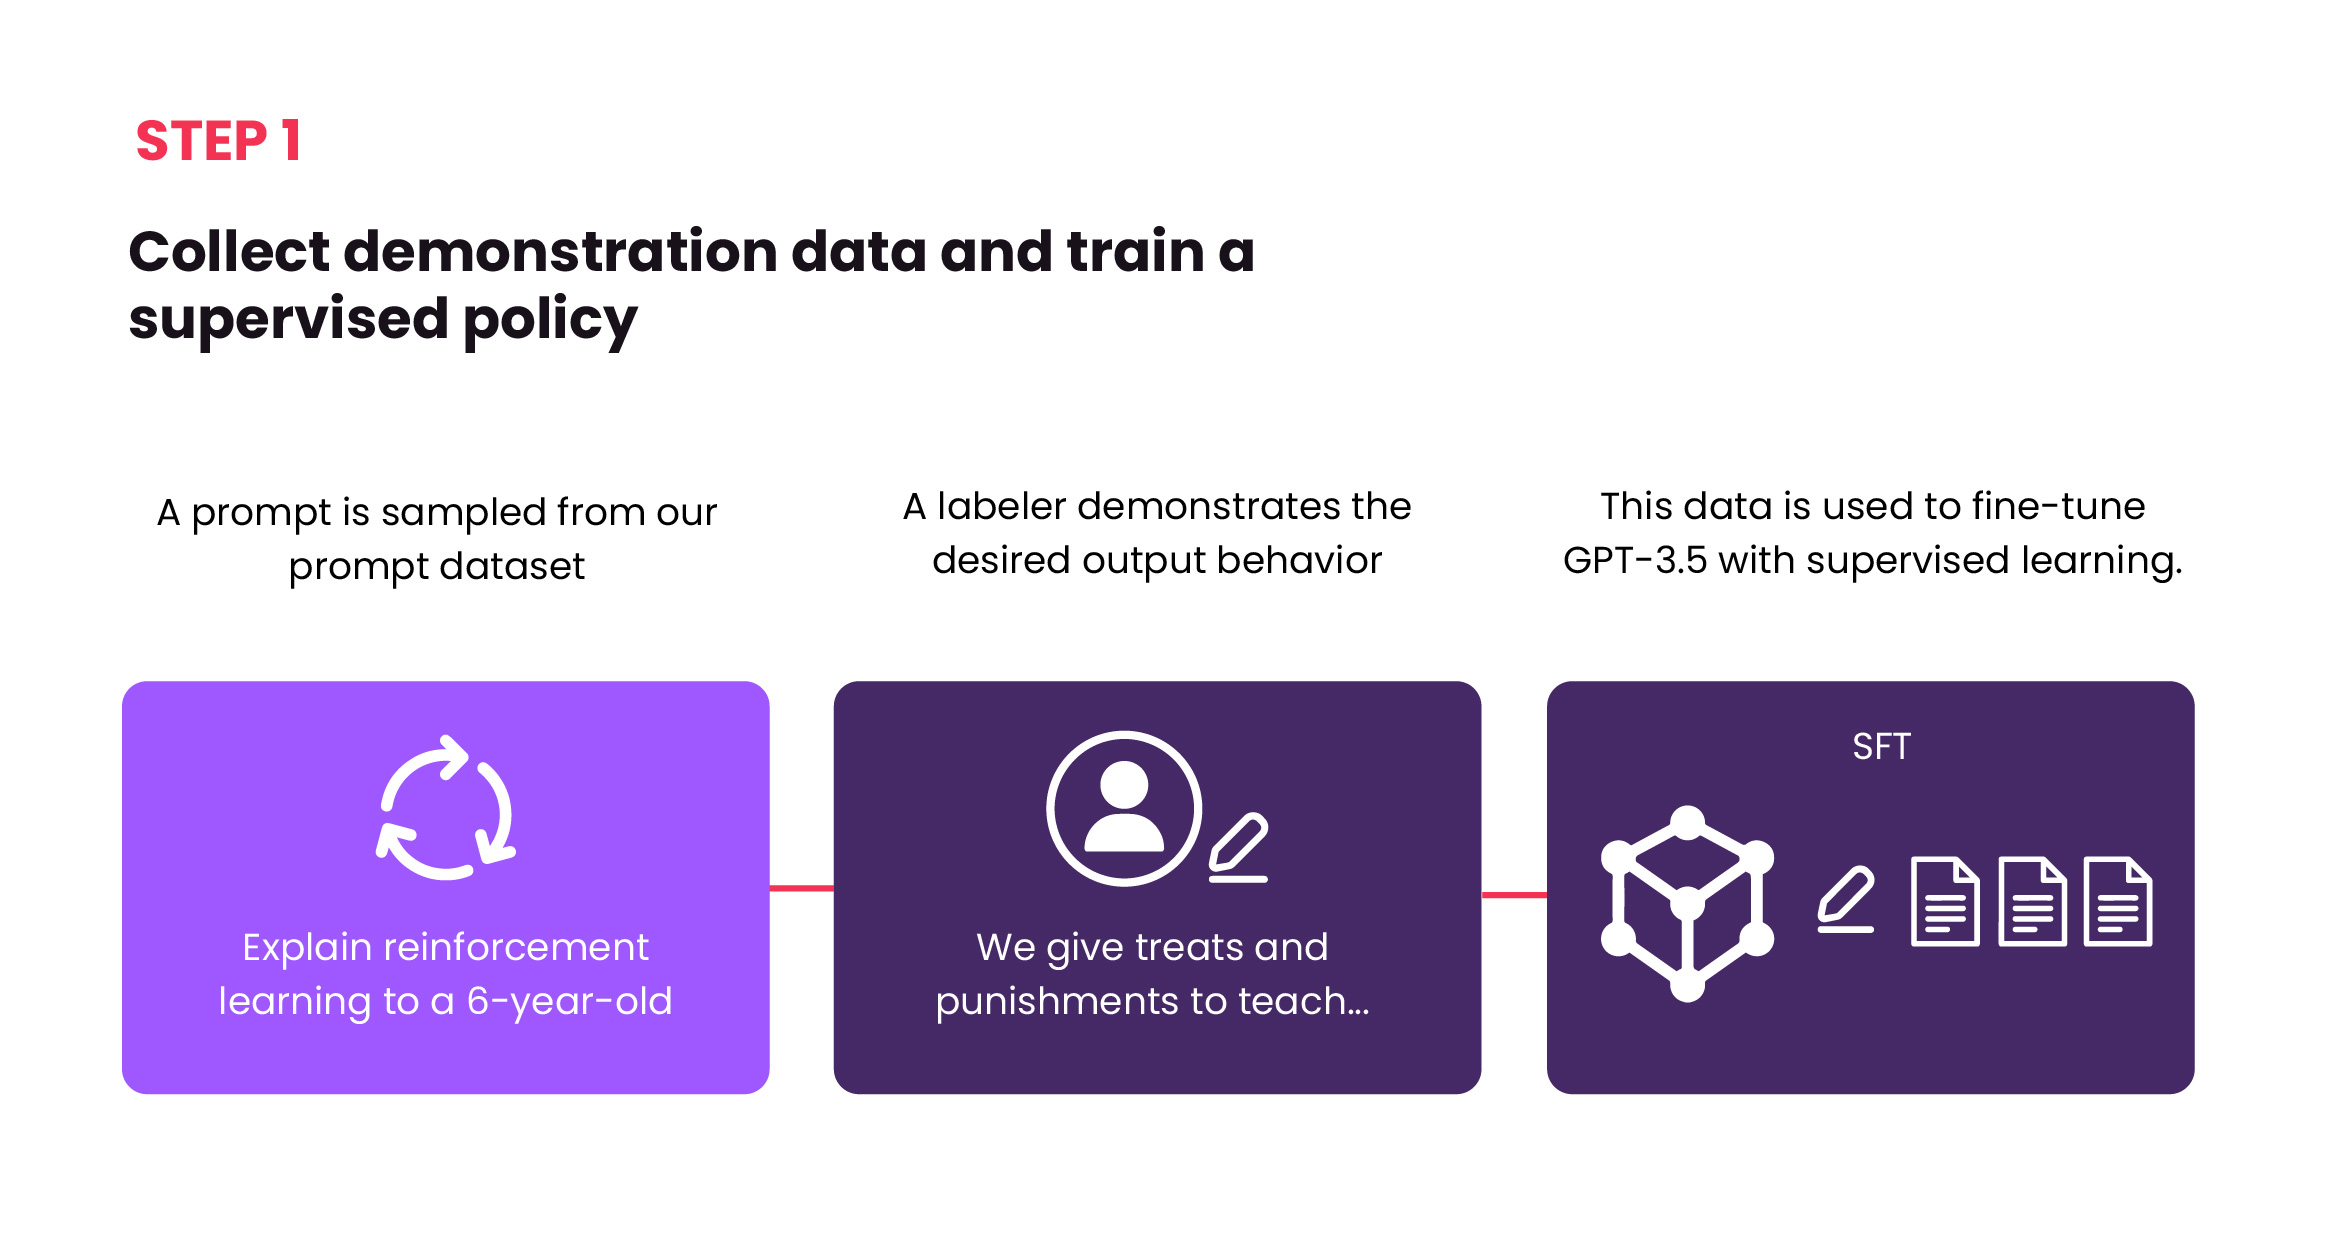
\includegraphics[width=0.8\linewidth,keepaspectratio]{chatgpt4}
			
			\end{center}		
			
			{\tiny (Ref: ChatGPT: training process, advantages, and limitations - By Sergio Soage, Machine Learning Engineer at Aivo)}
			
\end{frame}

%%%%%%%%%%%%%%%%%%%%%%%%%%%%%%%%%%%%%%%%%%%%%%%%%%%%%%%%%%%
\begin{frame}[fragile]\frametitle{Step 2}

\begin{itemize}
\item For a prompt, generate multiple responses from the fine-tuned model, one after another.
\item Human feedback provides a ranking of responses
\item This data is used to build Rewards Model (RM)
\end{itemize}	 

			\begin{center}
			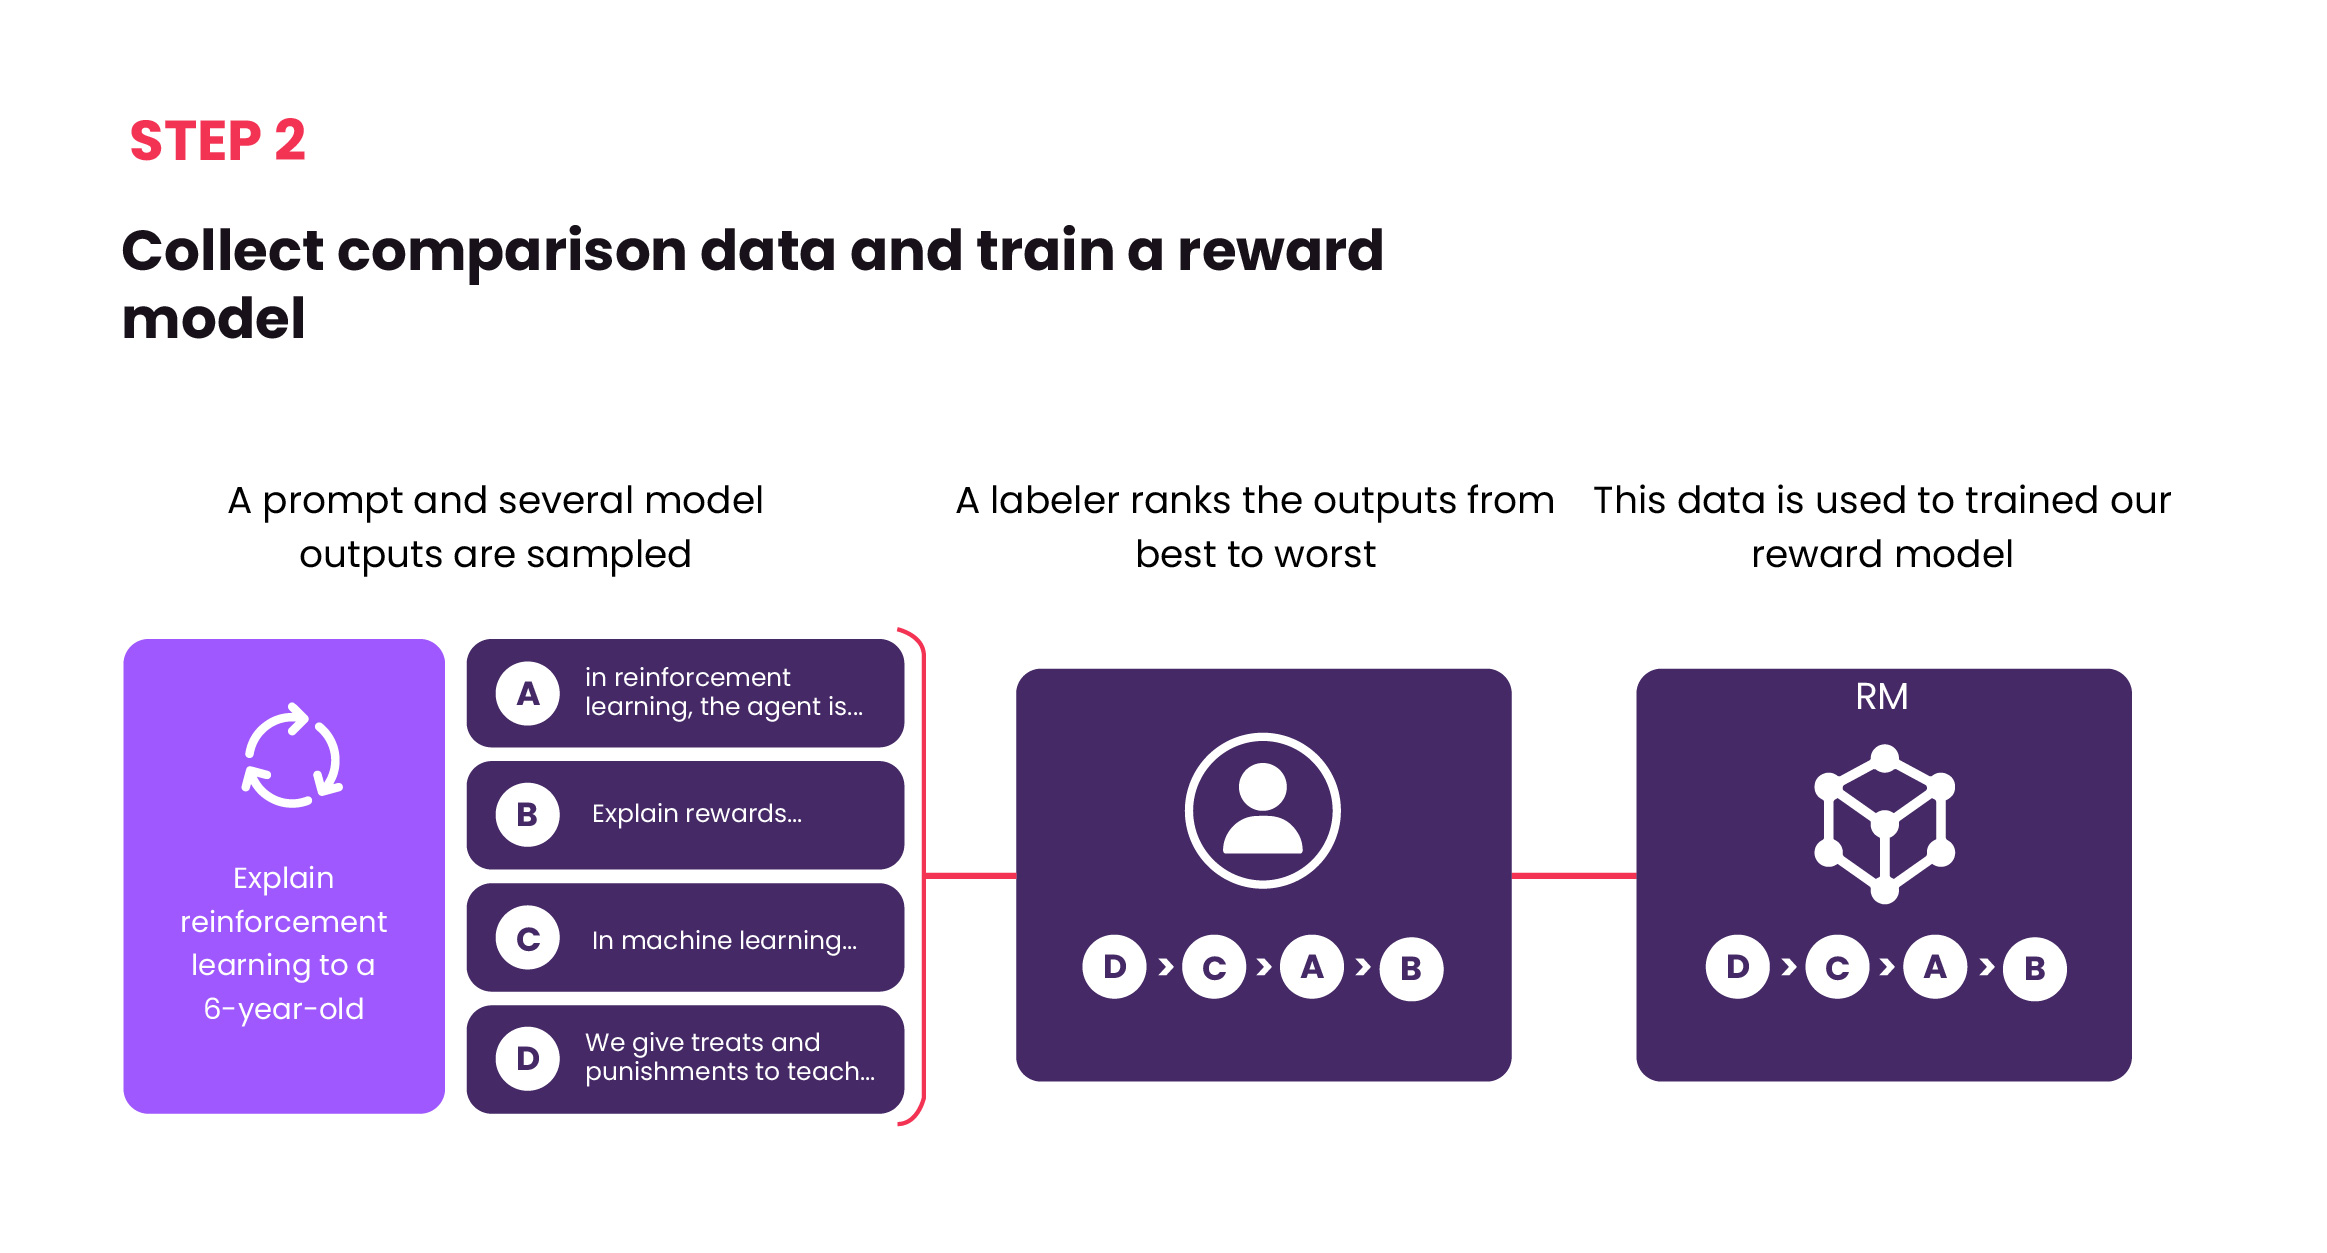
\includegraphics[width=0.8\linewidth,keepaspectratio]{chatgpt5}
			
			\end{center}		
			
			{\tiny (Ref: ChatGPT: training process, advantages, and limitations - By Sergio Soage, Machine Learning Engineer at Aivo)}
			
\end{frame}


% %%%%%%%%%%%%%%%%%%%%%%%%%%%%%%%%%%%%%%%%%%%%%%%%%%%%%%%%%%%
% \begin{frame}[fragile]\frametitle{Step 2: Manual Ranking}


			% \begin{center}
			% 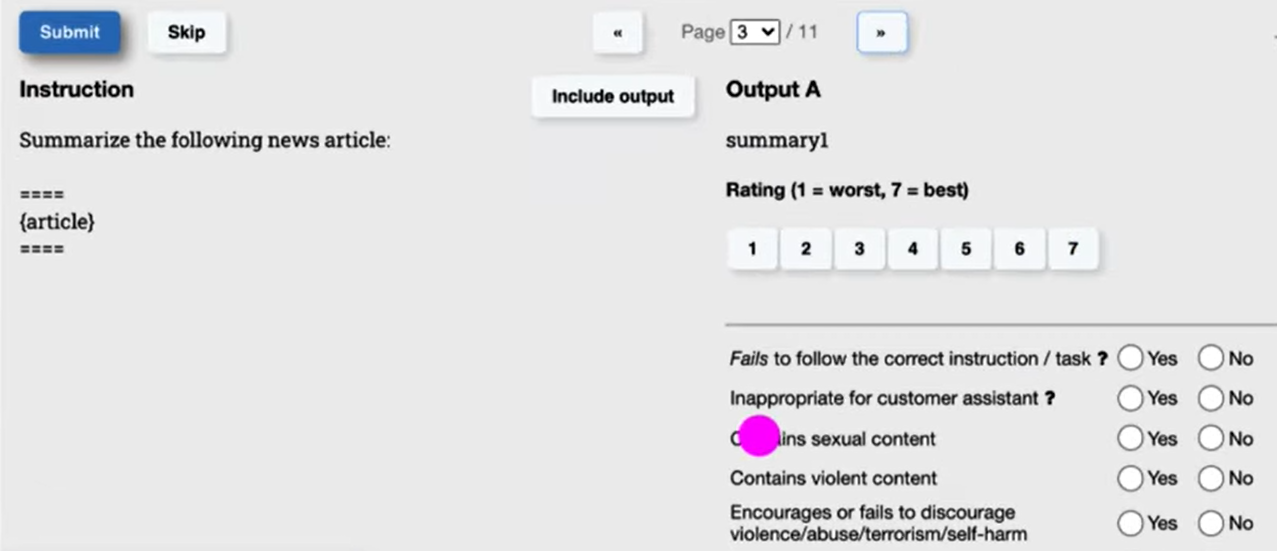
\includegraphics[width=\linewidth,keepaspectratio]{chatgpt10}
			
			% \end{center}		
			
			% {\tiny (Ref: ChatGPT - Explained! - CodeEmporium)}
			
% \end{frame}


%%%%%%%%%%%%%%%%%%%%%%%%%%%%%%%%%%%%%%%%%%%%%%%%%%%%%%%%%%%
\begin{frame}[fragile]\frametitle{Step 3}

\begin{itemize}
\item Take unseen prompt. Pass it through Proximal Policy Optimization (PPO) model which has been initialized with SFT. It generates a response (ie inferencing via SFT).
\item Calculate reward for that response via RM model. This reward is used to update the PPO model (loss function, back-propagation)
\end{itemize}	 

			\begin{center}
			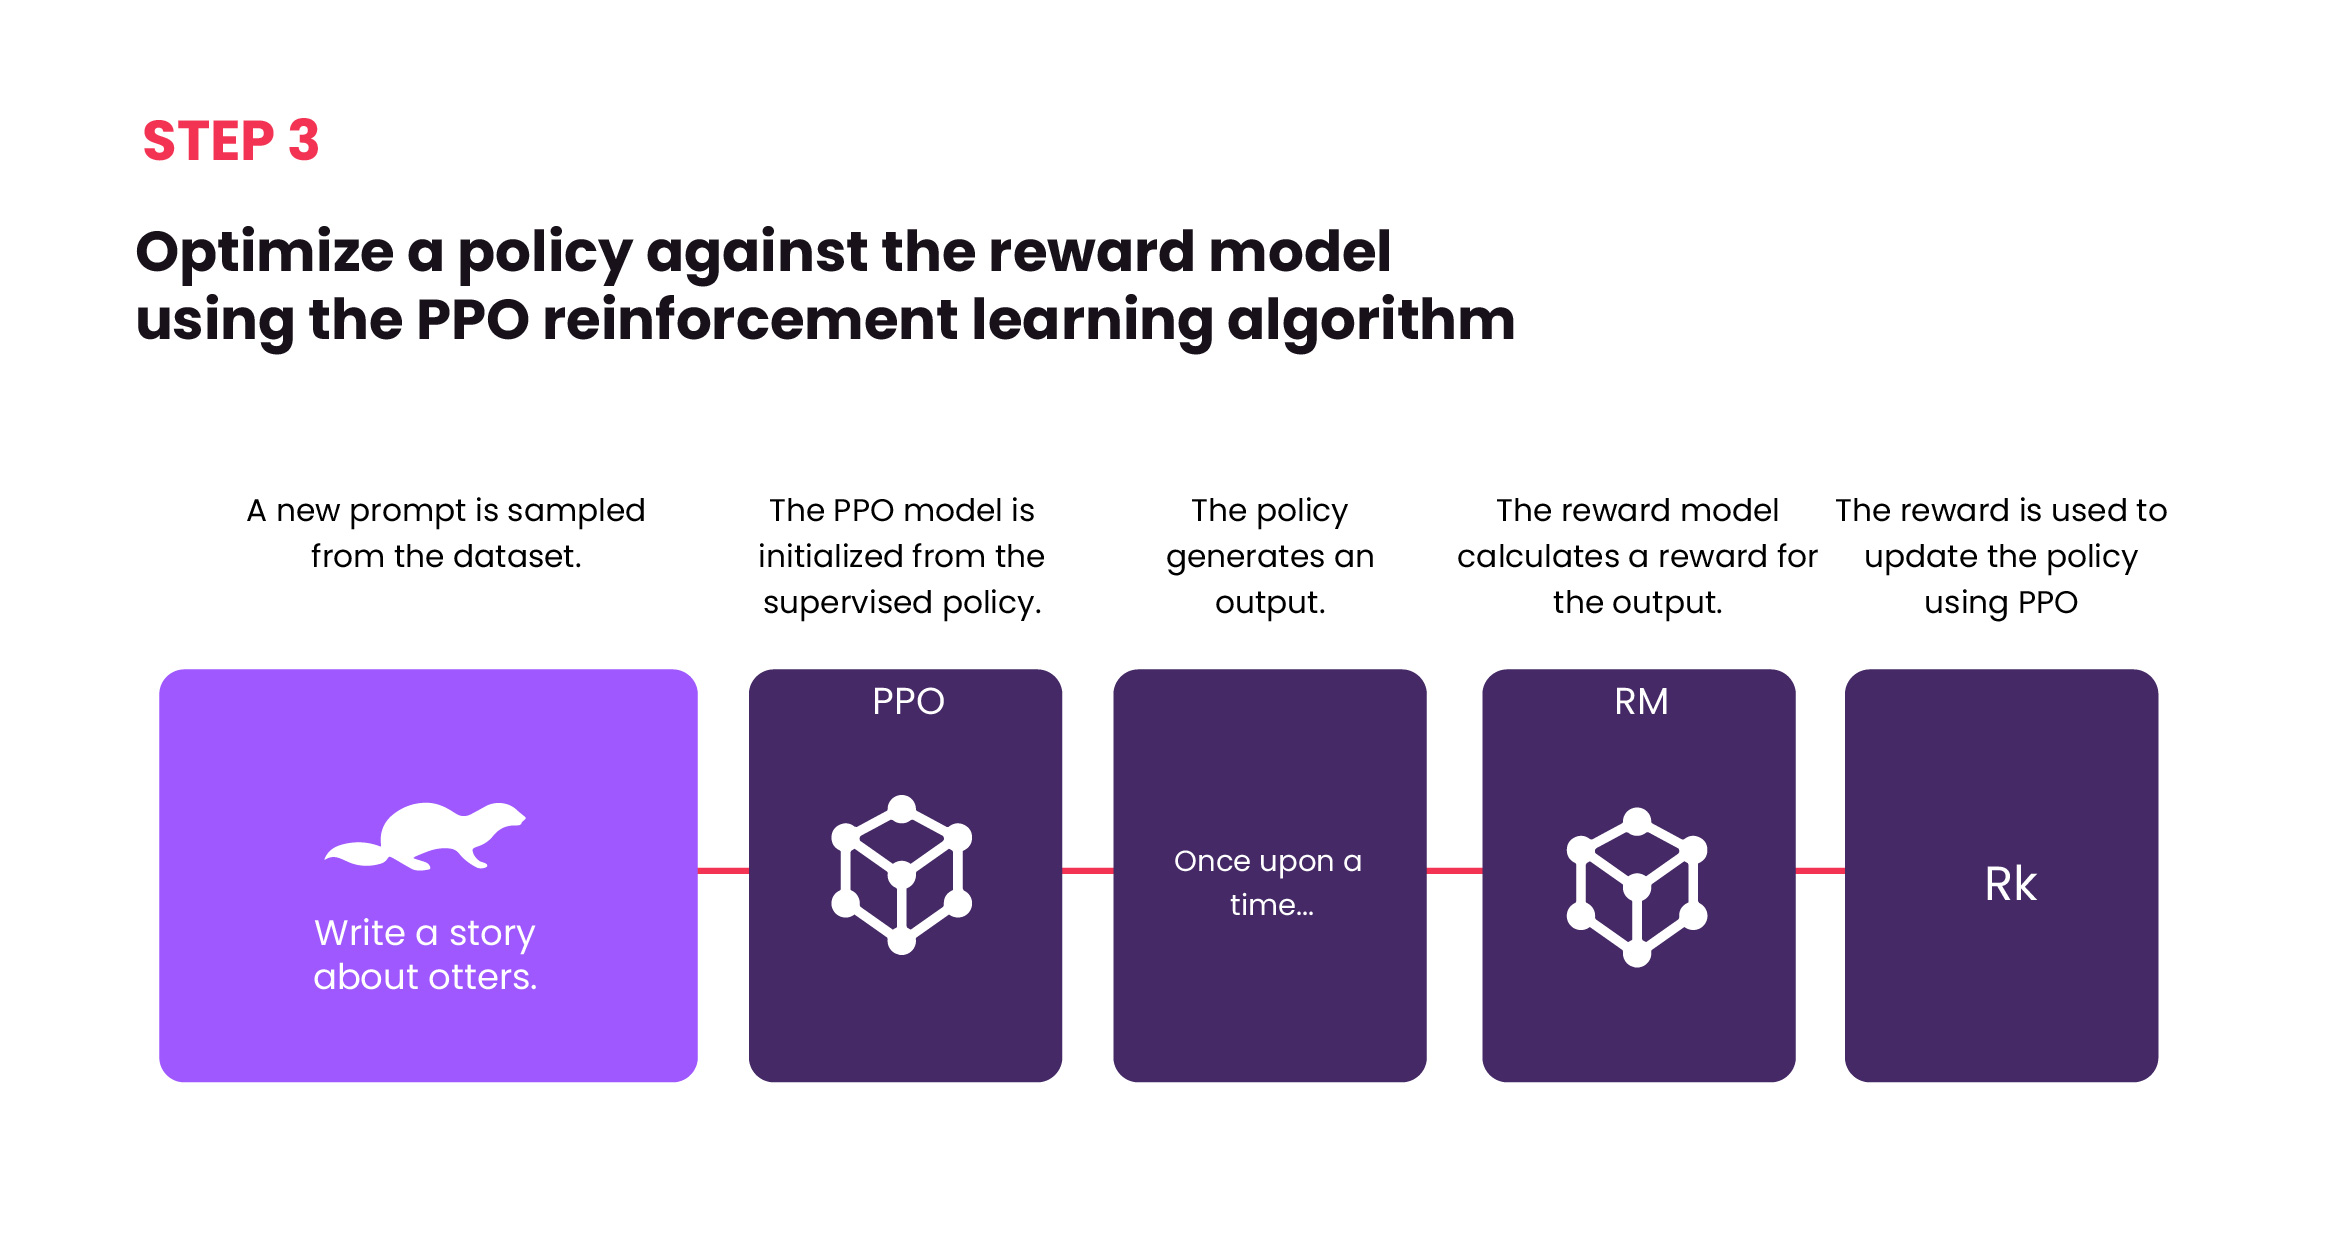
\includegraphics[width=0.8\linewidth,keepaspectratio]{chatgpt6}
			
			\end{center}		
			
			{\tiny (Ref: ChatGPT: training process, advantages, and limitations - By Sergio Soage, Machine Learning Engineer at Aivo)}
			
\end{frame}


%%%%%%%%%%%%%%%%%%%%%%%%%%%%%%%%%%%%%%%%%%%%%%%%%%%%%%%%%%%
\begin{frame}[fragile]\frametitle{Advantages}


\begin{itemize}
\item Creative Assistant, random-mix-ideas
\item Will replace mundane language tasks, How to articles, homeworks, etc
\item Supports more complex instructions, ``reasoning'' tasks
\end{itemize}	 

\end{frame}

%%%%%%%%%%%%%%%%%%%%%%%%%%%%%%%%%%%%%%%%%%%%%%%%%%%%%%%%%%%
\begin{frame}[fragile]\frametitle{Dis-advantages}


\begin{itemize}
\item Cannot replace humans for innovation, for which data does not exist already
\item Keeps ``hallucinating''
\item Tends to write plausible but incorrect content with confidence
\item Cannot get language structure right all the time, e.g try getting ghazal written
\end{itemize}	 

\end{frame}

%%%%%%%%%%%%%%%%%%%%%%%%%%%%%%%%%%%%%%%%%%%%%%%%%%%%%%%%%%%
\begin{frame}[fragile]\frametitle{Conclusion}



			\begin{center}
			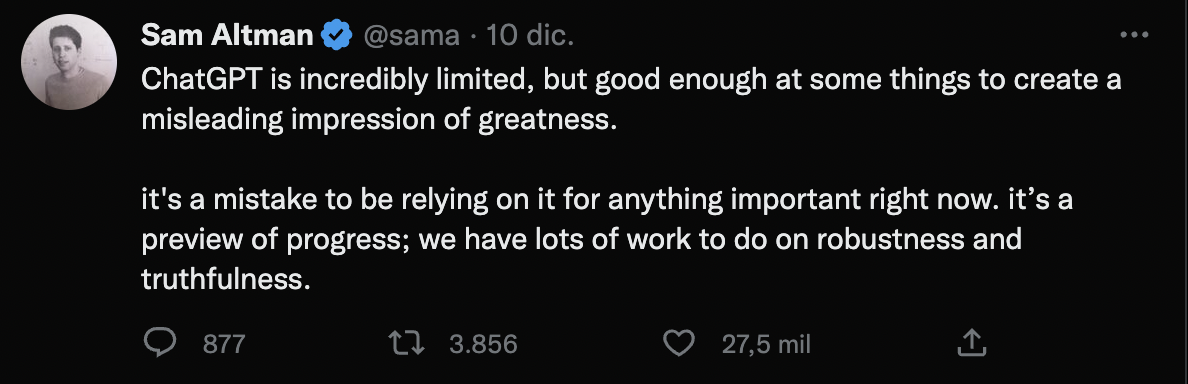
\includegraphics[width=\linewidth,keepaspectratio]{chatgpt7}
			
			\end{center}		
			
			{\tiny (Ref: ChatGPT: training process, advantages, and limitations - By Sergio Soage, Machine Learning Engineer at Aivo)}
			

\end{frame}